% $Header: /project/cl/Root/CVS/talks/iowa08/talk.tex,v 1.3 2008/01/31 14:11:37 stump Exp $

\documentclass[11pt]{beamer}

\usepackage{tikz}
\usepackage{pgflibraryarrows}
\usepackage{pgflibraryshapes}
\usepackage{pgfbaseimage}
\usepackage{proof}
\usepackage{url}

\newcommand{\Eq}[0]{\texttt{=}}
\newcommand{\Neq}[0]{\texttt{!=}}
\newcommand{\Qeq}[0]{\stackrel{?}{=}}
\newcommand{\bang}[0]{\texttt{!}}
\newcommand{\quant}[0]{\textit{Quant}}

\newcommand{\To}[0]{\Rightarrow}
\newcommand{\rn}[1]{\textsc{#1}}
\newcommand{\interp}[1]{[ \negthinspace [ #1 ] \negthinspace ]}

\newcommand{\seq}[3]{#1 \vdash #2 : #3}
%\newcommand{\aseq}[3]{ #2 : #3}
\newcommand{\aseq}[3]{ #1 \vdash #3}
%\newcommand{\aaseq}[3]{ #3}
\newcommand{\aaseq}[3]{ #1 \vdash #3}
\newcommand{\abseq}[3]{ #1 \vdash #3}

\newcommand{\ppp}[1]{\begin{tikzpicture}
\draw (-2,0) 
   node[fill=orange!40,ellipse,minimum height=1cm,minimum width=3cm](f) {proofs};
\draw (2,0)
   node[fill=blue!40,ellipse,minimum height=1cm,minimum width=3cm](g) {programs};
\draw[-latex',orange!40,very thick] (f.north) .. controls (-1,1) and (1,1) .. (g.north);
\draw[-latex',blue!40,very thick] (g.south) .. controls (1,-1) and (-1,-1) .. (f.south);
\draw (0,0) node {\Huge #1};
\end{tikzpicture}}


\mode<presentation>
{
  %\usetheme{Warsaw}
  % or ...

\usetheme{IowaCity}
%\usetheme{Edinburgh}

%  \setbeamercovered{transparent}
  % or whatever (possibly just delete it)
}


\usepackage[english]{babel}
% or whatever

\usepackage[latin1]{inputenc}
% or whatever

\usepackage{times}
\usepackage[T1]{fontenc}
% Or whatever. Note that the encoding and the font should match. If T1
% does not look nice, try deleting the line with the fontenc.

\title[Verified Tools in OpTT]
{Building Verified Language Tools in\\ Operational Type Theory}

\author{Aaron~Stump}

\institute[Computational Logic Center]
{
  Computational Logic Center\\
  Computer Science Department \\
  The University of Iowa\\
\ \\ 
\ \\ Thanks to Morgan Deters and Todd Schiller.
\ \\
\ \\
Funding from NSF CAREER. 
}

\pgfdeclareimage[height=2cm]{laundry}{laundry}
\pgfdeclareimage[height=3cm]{car}{repaired-car}

% If you have a file called "university-logo-filename.xxx", where xxx
% is a graphic format that can be processed by latex or pdflatex,
% resp., then you can add a logo as follows:

% \pgfdeclareimage[height=0.5cm]{university-logo}{university-logo-filename}
% \logo{\pgfuseimage{university-logo}}



% Delete this, if you do not want the table of contents to pop up at
% the beginning of each subsection:
%\AtBeginSubsection[]
%{
%  \begin{frame}<beamer>
%    \frametitle{Outline}
%    \tableofcontents[currentsection,currentsubsection]
%  \end{frame}
%}


% If you wish to uncover everything in a step-wise fashion, uncomment
% the following command: 

%\beamerdefaultoverlayspecification{<+->}

\begin{document}

\date{\ }

\begin{frame}[plain]
  \titlepage
\end{frame}

\date{WMM '08}

\begin{frame}
  \frametitle{From Meta-Theory to Tools}

\begin{itemize}
\item Mechanized meta-theory great.


\begin{center}
\pgfuseimage{laundry}
\end{center}


\item Verified language tools also great!


\begin{center}
\pgfuseimage{car}
\end{center}


\item The combination definitely the greatest.

\end{itemize}

\end{frame}


\begin{frame}
\frametitle{Meta-theory and Tools for LF}
\begin{itemize}
\item Paper meta-theory for LF \textcolor{blue}{[Harper+05],[Watkins+02]}.
\item Machine-checked meta-theory for LF \textcolor{blue}{[Urban+08]}.
\item Unverified tools for LF: \textsc{Twelf}, \textsc{flit}, \textsc{sc}, \textsc{lfsc}.
\item Verified tool (this talk): \textsc{Golfsock}.
\begin{itemize}
\item Verify that optimized LF checker builds type-correct LF.
\item Uses a declarative presentation of LF.
\item Still efficient, but much more trustworthy.
\item Partial verification.
\end{itemize}
\end{itemize}
\end{frame}

\begin{frame}[containsverbatim]
\frametitle{Incremental Checking}
\begin{itemize}
\item Basic idea: interleave parsing and checking \textcolor{blue}{[Stump08]}.
\item Combine with bidirectional type checking.
\begin{itemize}
\item Synthesizing: $\Gamma \vdash t \Rightarrow T$.
\item Checking: $\Gamma \vdash t \Leftarrow T$.
\end{itemize}
\item ASTs built for subterms iff they will appear in the type $T$.

E.g., 

\begin{verbatim}
(refl x+y) => x+y == x+y
\end{verbatim}

\begin{itemize}
\item AST must be built for \texttt{x+y}.
\item But not \texttt{(refl x+y)}.
\end{itemize}

\item C++ implementation: small footprint, fastest checker I know.

\end{itemize}
\end{frame}

\begin{frame}
\frametitle{A Need for Correctness}

\begin{itemize}
\item LF with Side Conditions (LFSC) proposed for SMT.
\begin{itemize}
\item Satisfiability Modulo Theories.
\item SMT solvers check large formulas, produce big proofs.
\item Must check proofs efficiently.
\item LFSC provides flexible intermediate proof language.
\item Extends LF with computational side conditions. 
\end{itemize}
\item Problems with C++ checker:
\begin{itemize}
\item Lack of memory safety => many days with \texttt{valgrind}.
\item Optimizations reduce trustworthiness.
\end{itemize}
\item As features are added to checker, trust diminishes.
\item Additional assurance is required.
\end{itemize}
\end{frame}

\begin{frame}
\frametitle{Towards A Verified LFSC Checker}
\begin{itemize}
\item \textsc{Golfsock} (``\textsc{Guru} LFSC'').
\begin{itemize}
\item \textsc{Guru} is a verified functional programming language.
\item Supports mutable state, non-termination, I/O.
\item Verification via dependent types, induction proofs.
\item Type/proof checker, compiler to efficient C code.
\item Beating native code \textsc{OCaml} on small testcases.
\end{itemize}
\item Status:
\begin{itemize}
\item Incremental LF checking implemented.
\item Running reasonably fast: 50\% slower than C++ version.
\item Specification: ASTs we build are type correct LF.
\item Expressed with dependent types, declarative LF.
\item 4300 lines code, proof; 13000 lines standard library (e.g., tries).
\end{itemize}
\end{itemize}
\end{frame}

\begin{frame}
\frametitle{\textsc{Guru} and Operational Type Theory}
\begin{itemize}
\item \textsc{Guru} implements Operational Type Theory (OpTT).
\item OpTT is new type theory intended to:
\begin{itemize}
\item Combine programming, theorem proving (cf. ATS, Epigram, Ynot).
\item Allow general recursion, other effects.
\item Retain sound logic.
\item Retain decidability of type checking.
\item Support external reasoning about dependently typed programs.
\item Support compilation to efficient executables.
\end{itemize}
\item Critical design idea: separate different reductions.
\begin{itemize}
\item Reduction for definitional equality ($\equiv$).
\item Reduction for programs.
\item Normalization (aka, cut elimination) for proofs.
\end{itemize}
\end{itemize}
\end{frame}

\begin{frame}
\frametitle{Rejection of Curry-Howard}
\begin{itemize}
\item Proofs $\neq$ Programs, Formulas $\neq$ Types.

\ 

\begin{center}
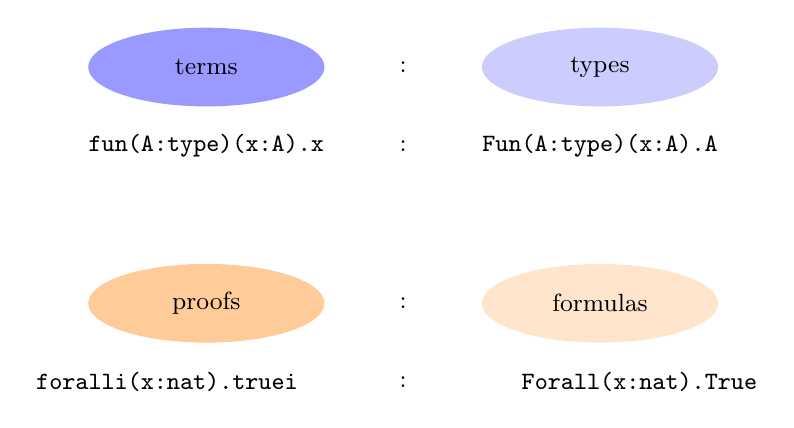
\begin{tikzpicture}
\small
\draw (-2.5,2)
   node[fill=blue!40,ellipse,minimum height=1cm,minimum width=3cm] {terms};
\draw (2.5,2)
   node[fill=blue!20,ellipse,minimum height=1cm,minimum width=3cm] {types};
\draw (0,2) node { :};
\draw (-2.5,1) node{\texttt{fun(A:type)(x:A).x}};
\draw (2.5,1) node{\texttt{Fun(A:type)(x:A).A}};
\draw (0,1) node { :};

\draw (-2.5,-1) 
   node[fill=orange!40,ellipse,minimum height=1cm,minimum width=3cm] {proofs};
\draw (2.5,-1) 
   node[fill=orange!20,ellipse,minimum height=1cm,minimum width=3cm] {formulas};
\draw (0,-1) node { :};
\draw (-3,-2) node{\texttt{foralli(x:nat).truei}};
\draw (3,-2) node{\texttt{Forall(x:nat).True}};
\draw (0,-2) node { :};
\end{tikzpicture}
\end{center}

\item Otherwise non-terminating programs $=$ unsound proofs.

\end{itemize}
\end{frame}

\begin{frame}
\frametitle{Rejection of Conversion}
\begin{itemize}
\item Definitional equality ($\equiv$) cannot include program reduction.

\item Otherwise type checking undecidable.

\item Adopt a very weak $\equiv$ ($\equiv_\alpha$, definitions, sugar).

\item Constrast with strong conversion relations.
\begin{itemize}
\item CIC: $\equiv$ includes $\equiv_\beta$, terminating recursion.

\item CCIC: $\equiv$ uses decision procedures, hypotheses.

\end{itemize}

\item With conversion, lose definitional transparency.
\item Typing holds modulo $\equiv$, but not other operations.
\begin{itemize}
\item $\Gamma \vdash t : T$ \ \ => \ \ $\Gamma' \vdash t' : T'$ with $\Gamma \equiv \Gamma'$, $t \equiv t'$, $T \equiv T'$.
\item Rewriting modulo $\equiv_\beta$ only recently decidable \textcolor{blue}{[Stirling06]}.
\item In Coq, many tactics do not work modulo $\equiv$.
\item In \textsc{Guru}, all tactics work modulo $\equiv$.
\end{itemize}

\end{itemize}
\end{frame}

\begin{frame}
\frametitle{Operational Equality}
\begin{itemize}
\item Due to weak $\equiv$, need casts in code (and proofs):

\ 

$\infer{\texttt{cast\ t\ by\ P} : {\texttt{T}_2}}
      {\texttt{t} : \texttt{T}_1 & 
        \texttt{P} : \texttt{\{T}_1\texttt{ = T}_2\texttt{\}}}$

\ 

\item Reasoning about code with casts tedious in other systems.

\item In OpTT, reason about unannotated programs.

\begin{itemize}
\item Propositional equality \texttt{\{ t = t' \}} holds if $t \downarrow t'$.
\item No type annotations, casts, proofs in \texttt{t}, \texttt{t'}.
\item No \emph{specificational data}.
\item Vastly simplifies external reasoning about code.
\item Annotations dropped by definitional equality.
\end{itemize}
\end{itemize}
\end{frame}

\begin{frame}[containsverbatim]
\frametitle{Example: Vector Append}
\footnotesize
\begin{verbatim}
Inductive vec : Fun(A:type)(n:nat).type :=
  vecn : Fun(A:type).<vec A Z>
| vecc : Fun(A:type)(spec n:nat)(a:A)(l:<vec A n>).
              <vec A (S n)>.

vec_append : Fun(A:type)(spec n m:nat)
                (l1 : <vec A n>)(l2 : <vec A m>).
                <vec A (plus n m)>

vec_append_assoc : 
  Forall(A:type)(n1 : nat)(l1 : <vec A n1>)
        (n2 n3 : nat)(l2 : <vec A n2>)(l3 : <vec A n3>).
  { (vec_append (vec_append l1 l2) l3) =
    (vec_append l1 (vec_append l2 l3)) }
\end{verbatim}

\end{frame}

\begin{frame}
\frametitle{Functional Modeling and Ownership}
\begin{itemize}
\item Following \textcolor{blue}{[Swierstra+07]}: awkwardness => modeling school.
\item Awkward squad modeled functionally.
\begin{itemize}
\item Standard input is a list of chars.
\item \texttt{getc()} is head.
\item Mutable arrays of length $n$ are vectors of length $n$.
\item \texttt{read} and \texttt{write} are pure, $O(n)$ operations.
\end{itemize}
\item Reason about code using functional model.
\item Replace during compilation with non-functional implementation.
\item Restrict usage for soundness (monads or linear types).
\item \textsc{Guru} uses linear types.
\begin{itemize}
\item Fit well with \emph{ownership types}.
\item \textsc{Guru} statically tracks ownership of all data.
\item Enables reference counting for memory management.
\item Function inputs \texttt{unowned}, \texttt{owned}, \texttt{unique}, or \texttt{unique\_owned}.
\end{itemize}
\end{itemize}
\end{frame}

\begin{frame}
\frametitle{\textsc{Golfsock}: Symbols}
\begin{itemize}
\item Incrementally consume textual input, type check LF.
\item LF variables (constants) implemented as 32-bit words.
\begin{itemize}
\item Implementation with \texttt{nat} too slow.
\item Words are functionally modeled as \texttt{<vec bool 32>}.
\item Trusted operations: increment, equality check, create 0.
\item Reason via model, also via conversion to \texttt{nat}.
\end{itemize}
\item Symbol table maps strings (lists of chars) to (var, type) pairs.
\item Symbol table implemented as a trie.
\item Mutable char-indexed arrays of subtries at each node.
\end{itemize}
\end{frame}

\begin{frame}
\frametitle{\textsc{Golfsock}: LF derivations}
\begin{itemize}
\item Code ``builds'' specificational LF derivations.
\item For $\Gamma \vdash t \Leftarrow T$ (or $\Gamma \vdash t \Rightarrow T$), we build \texttt{<deriv G t T>}.
\item Context encoded as a list of (var,type) pairs.
\item Must map the symbol table to context.
\begin{itemize}
\item Difficult.
\item Must prove lemmas like trie membership => context membership.
\item Resulting context is not ordered.
\item Phrase typing rules for unordered contexts.
\item Ok, because vars uniquely named.
\end{itemize}
\end{itemize}
\end{frame}

\begin{frame}
\frametitle{Empirical Results}
\begin{figure}
\footnotesize
\begin{center}
\begin{tabular}{|l|l|l|l|l|l|l|l|}
\hline
benchmark & size (MB) & C++ impl & \textsc{Golfsock} & \textsc{Twelf}
\\
\hline
cnt01e
&
2.6
&
1.3
&
2.0
&
14.0 
\\
tree-exa2-10
&
3.1
&
1.7
&
2.5
&
18.6
\\
cnt01re
&
4.6
&
2.4
&
3.6
&
218.4
\\
toilet\_02\_01.2
&
11
&
5.8
&
8.8
&
1143.8
\\
1qbf-160cl.0
&
20
&
10.0
&
14.1
&
timeout
\\
tree-exa2-15
&
37
&
19.9
&
31.2
&
timeout 
\\
toilet\_02\_01.3
&
110
&
58.6
&
89.7
&
exception 
\\
\hline
\end{tabular}
\end{center}
\caption{\label{fig:qbf}Checking times in seconds for QBF benchmarks}
\end{figure}

\begin{itemize}
\item Good, since some optimizations not implemented.
\end{itemize}

\end{frame}

\begin{frame}
\frametitle{Conclusion}
\begin{itemize}
\item \textsc{Golfsock}: towards verified, efficient language tools.
\item OpTT makes this easier:
\begin{itemize}
\item Not required \emph{a priori} to prove termination.
\item Reason about code with annotations dropped.
\item Use dependent types for big functions (\texttt{check}, 1200 lines).
\item Supports functional modeling.
\end{itemize}

\item Onward towards verified, efficient software!
\end{itemize}

\begin{center}
\large
\textcolor{blue}{\url{www.guru-lang.org}}
\end{center}

\end{frame}

\end{document}

